% !TeX encoding = UTF-8

%% ------------------------------------------------------------------------
%% Copyright (C) 2021,2022 SJTUG
%% 
%% SJTUBeamer Example Document by SJTUG
%% 
%% SJTUBeamer Example Document is licensed under a
%% Creative Commons Attribution-NonCommercial-ShareAlike 4.0 International License.
%% 
%% You should have received a copy of the license along with this
%% work. If not, see <http://creativecommons.org/licenses/by-nc-sa/4.0/>.
%%
%% For a quick start, check out src/doc/sjtubeamerquickstart.tex
%% Join discussions: https://github.com/sjtug/SJTUBeamer/discussions
%% -----------------------------------------------------------------------

\documentclass[xcolor=table,dvipsnames,svgnames,aspectratio=169]{ctexbeamer}
% 可以通过 fontset=macnew / fontset=ubuntu / fontset=windows 选项切换字体集

\usepackage{tikz}
\usepackage[normalem]{ulem}
\usetikzlibrary{arrows}
\usepackage{amsmath}
\usepackage{mflogo}
\usepackage{graphicx}
\usepackage{ccicons}
\usepackage{hologo}
\usepackage{colortbl}
\usepackage{shapepar}
\usepackage{hyperxmp}
\usepackage{booktabs}
\usepackage{qrcode}
\usepackage{listings}
\usepackage{tipa}
\usepackage{multicol}
\usepackage{datetime2}
\usepackage{fontawesome5}
\usepackage{hyperref}

% 参考文献设置,使用 style=gb7714-2015 样式为标准顺序编码制,
% 使用 style=gb7714-2015ay 样式可以改为著者-出版年制。
\usepackage[backend=biber,style=gb7714-2015]{biblatex}
\addbibresource{thesis.bib}

\graphicspath{{figures/}}

\hypersetup{
  pdfsubject = {上海交通大学图书馆专题培训讲座},
  pdfauthor = {Alexara Wu},
  pdfcopyright = {Licensed under CC-BY-SA 4.0. Some rights reserved.},
  pdflicenseurl = {http://creativecommons.org/licenses/by-sa/4.0/},
  unicode = true,
  psdextra = true,
  pdfdisplaydoctitle = true
}

\pdfstringdefDisableCommands{
  \let\\\relax
  \let\quad\relax
  \let\hspace\@gobble
}

\renewcommand{\TeX}{\hologo{TeX}}
\renewcommand{\LaTeX}{\hologo{LaTeX}}
\newcommand{\BibTeX}{\hologo{BibTeX}}
\newcommand{\XeTeX}{\hologo{XeTeX}}
\newcommand{\pdfTeX}{\hologo{pdfTeX}}
\newcommand{\LuaTeX}{\hologo{LuaTeX}}
\newcommand{\MiKTeX}{\hologo{MiKTeX}}
\newcommand{\MacTeX}{Mac\hologo{TeX}}
\newcommand{\beamer}{\textsc{beamer}}
\newcommand{\XeLaTeX}{\hologo{Xe}\kern-.13em\LaTeX{}}
\newcommand{\pdfLaTeX}{pdf\LaTeX{}}
\newcommand{\LuaLaTeX}{Lua\LaTeX{}}

\def\TeXLive{\TeX{} Live}
\let\TL=\TeXLive
\newcommand{\SJTUThesis}{\textsc{SJTUThesis}}
\newcommand{\SJTUThesisVersion}{1.1.0}
\newcommand{\SJTUThesisDate}{2022/3/26}
\newcommand{\SJTUBeamer}{\textsc{SJTUBeamer}}
\newcommand{\SJTUBeamerVersion}{3.0.0}
\newcommand{\SJTUBeamerDate}{2022/11/22}

\newcommand\link[1]{\href{#1}{\faLink}}
\newcommand\pkg[1]{\texttt{#1}}

\def\cmd#1{\texttt{\color{structure}\footnotesize $\backslash$#1}}
\def\env#1{\texttt{\color{structure}\footnotesize #1}}
\def\cmdxmp#1#2#3{\small{\texttt{\color{structure}$\backslash$#1}\{#2\}
\hspace{1em}\\ $\Rightarrow$\hspace{1em} {#3}\par\vskip1em}}

\lstset{
  language=[LaTeX]TeX,
  basicstyle=\ttfamily\footnotesize,
  tabsize=2,
  keywordstyle=\bfseries\ttfamily\color{cprimary},
  commentstyle=\sl\ttfamily\color[RGB]{100,100,100},
  stringstyle=\ttfamily\color[RGB]{50,50,50},
  extendedchars=true,
  breaklines=true,
}

\usetheme[maxplus]{sjtubeamer}
% 使用 maxplus/max/min 切换标题页样式
% 使用 red/blue 切换主色调
% 使用 light/dark 切换亮/暗色模式
% 使用外样式关键词以获得不同的边栏样式
%   miniframes infolines  sidebar
%   default    smoothbars split	 
%   shadow     tree       smoothtree
% 使用 topright/bottomright 切换徽标位置
% 使用逗号分隔列表以同时使用多种选项

% \tikzexternalize[prefix=build/]
% 如果您需要缓存 tikz 图像,请取消注释上一行,并在编译选项中添加 -shell-escape。

\author{答辩人:刘思雨}
\institute[SJTU-PLV]{导师:汪宇霆}
\date{\the\year 年 \the\month 月}
\subject{LaTeX, 论文排版, SJTUThesis}

\title[中期答辩] % 页脚显示标题
{\textbf{中期答辩}} % 首页标题

\subtitle{基于静态单赋值中间语言的函数式编译器验证方法}

\begin{document}

% 使用节目录
\AtBeginSection[]{
  \begin{frame}
    %% 使用传统节目录,也可以将 subsectionstyle=... 换成 hideallsubsections 以隐藏所有小节信息
    \tableofcontents[currentsection,subsectionstyle=show/show/hide]
    %% 或者使用节页
    % \sectionpage
  \end{frame}
}

% 使用小节目录
\AtBeginSubsection[]{		       % 在每小节开始
  \begin{frame}
    %% 使用传统小节目录
    \tableofcontents[currentsection,subsectionstyle=show/shaded/hide]
    %% 或者使用小节页
    % \subsectionpage
  \end{frame}
}

\maketitle

\begin{frame}{研究课题概述}
  \begin{itemize}
    \item 延续传递风格(CPS)是函数式编译器中常用的中间语言,有利于控制流分析。
    \item 静态单赋值(SSA)是主流编译器常用的中间语言,有利于数据流分析。
    \item SSA程序可以用函数式程序表示。
    \item 目前\textcolor{Maroon}{没有}从CPS到SSA经过形式化验证的转换。
  \end{itemize}
  \begin{figure}
    \centering
    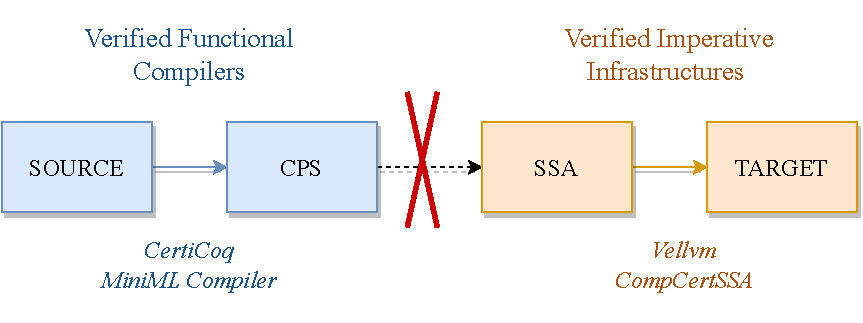
\includegraphics[width=0.7\linewidth]{figures/Motivation.drawio.pdf}
    \label{fig:moti1}
  \end{figure}
\end{frame}

\begin{frame}{研究课题概述}
  \begin{itemize}
    \item 实现并验证CPS到SSA语言的转换算法。
    \item 可以使经过形式化验证的函数式语言编译器复用基于SSA语言的优化。
  \end{itemize}
  \begin{figure}
    \centering
    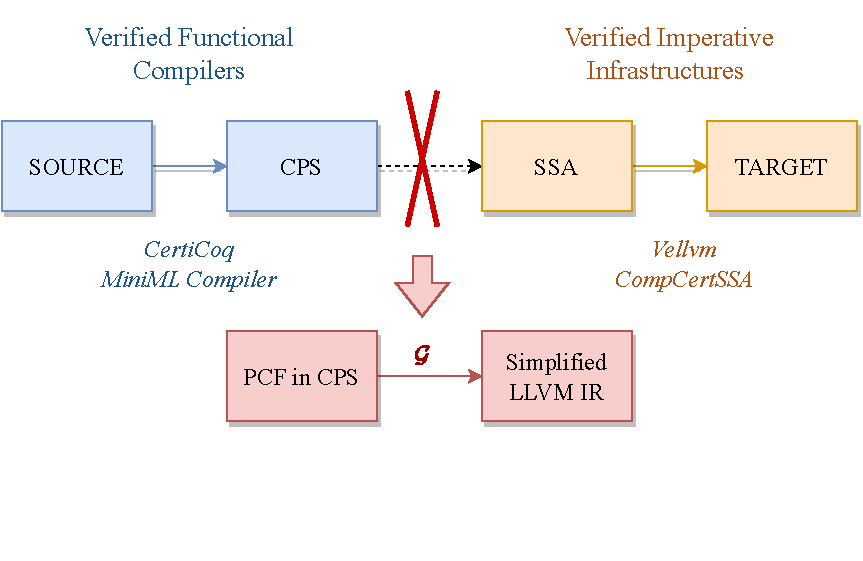
\includegraphics[width=0.7\linewidth]{figures/partial.drawio.pdf}
    \label{fig:moti2}
  \end{figure}  
\end{frame}


\begin{frame}{目录}
  \tableofcontents[hideallsubsections]	% 隐藏所有小节信息
\end{frame}

% !TeX encoding = UTF-8
% !TeX root = ../main.tex

%% ------------------------------------------------------------------------
%% Copyright (C) 2021,2022 SJTUG
%% 
%% SJTUBeamer Example Document by SJTUG
%% 
%% SJTUBeamer Example Document is licensed under a
%% Creative Commons Attribution-NonCommercial-ShareAlike 4.0 International License.
%% 
%% You should have received a copy of the license along with this
%% work. If not, see <http://creativecommons.org/licenses/by-nc-sa/4.0/>.
%% -----------------------------------------------------------------------

\section{研究进展}

\begin{frame}{研究工作进展}
  本课题研究工作按计划有序开展:
  \vspace{2ex}
  \begin{itemize}
    \item 定义\textcolor{Maroon}{源语言}及\textcolor{Maroon}{目标语言}。
      \begin{itemize}
        \item 使用\textcolor{Maroon}{PCF}(Programming Computable Functions)作为源程序语言。
        \item 将直接风格PCF的源程序进行CPS转换。
        \item 使用简化版的LLVM IR作为目标SSA语言。
      \end{itemize}
    \item \textcolor{Maroon}{CPS到SSA}的转换算法设计及实现。
    \item 用模拟技术对转换算法进行正确性\textcolor{Maroon}{验证}。
  \end{itemize}
\end{frame}

\begin{frame}{CPS $\Rightarrow$ SSA转换算法}
  定义函数\textcolor{Maroon}{$\mathcal{G}$}:
  \begin{enumerate}
    \item \textcolor{MidnightBlue}{初始:} CPS程序是待转换的源程序,SSA程序只有一个空的主函数。
    \item \textcolor{MidnightBlue}{$\mathcal{G}$递归翻译CPS程序:}
    \begin{itemize}
        \item 将新生成的程序组成部分(基本块,指令等)放入SSA程序。
        \item 更新函数的参数。
    \end{itemize}
    \item \textcolor{MidnightBlue}{转换完成:} 返回当前的SSA程序。  
\end{enumerate}
\vspace{1ex}
\small
\begin{columns}[c]
  \textcolor{MidnightBlue}{部分程序结构转换:}
  \begin{column}{0.6\textwidth}
  % \centering
  \begin{columns}
    \column{0.6\columnwidth}
    变量绑定 \\
    延续 \\
    多处变量应用到同一延续上 \\
    \column{0.05\columnwidth}
    $\Rightarrow$ \\
    $\Rightarrow$ \\
    $\Rightarrow$ \\
    \column{0.3\columnwidth}
    对新变量赋值 \\
    新的基本代码块 \\
    $\Phi$节点 \\
  \end{columns}
\end{column}
\end{columns}

\end{frame}




\section{研究成果}

\begin{frame}{研究工作进展}
    本课题研究工作按计划有序开展:
    \begin{itemize}
      \item 定义源程序语言及目标程序语言。
      \item 实现直接风格源语言的CPS转换。
      \item CPS到SSA的转换算法设计及实现。
      \item 用模拟技术对两步转换进行正确性验证。
      \item 将SSA程序编译到LLVM IR。
    \end{itemize}
  \end{frame}



% \include{contents/basis}
% \include{contents/thesis}
% % !TEX root = ../main.tex

\chapter{全文总结} \label{ch:summary}

\section{主要结论}

\section{研究展望}


% \begin{frame}
%   \frametitle{参考文献}
%   \printbibliography[heading=none]
% \end{frame}

\makebottom

\end{document}
